% !TEX TS-program = pdflatex
% !TEX encoding = UTF-8 Unicode

% This is a simple template for a LaTeX document using the "article" class.
% See "book", "report", "letter" for other types of document.

\documentclass[11pt]{article} % use larger type; default would be 10pt

\usepackage[utf8]{inputenc} % set input encoding (not needed with XeLaTeX)


%%% PAGE DIMENSIONS
\usepackage{geometry} % to change the page dimensions
\geometry{a4paper} % or letterpaper (US) or a5paper or....


\usepackage{graphicx} % support the \includegraphics command and options

% \usepackage[parfill]{parskip} % Activate to begin paragraphs with an empty line rather than an indent

%%% PACKAGES
\usepackage{booktabs} % for much better looking tables
\usepackage{array} % for better arrays (eg matrices) in maths
\usepackage{paralist} % very flexible & customisable lists (eg. enumerate/itemize, etc.)
\usepackage{verbatim} % adds environment for commenting out blocks of text & for better verbatim
\usepackage{subfig} % make it possible to include more than one captioned figure/table in a single float
\usepackage{cite}
% These packages are all incorporated in the memoir class to one degree or another...

%%% HEADERS & FOOTERS
\usepackage{fancyhdr} % This should be set AFTER setting up the page geometry
\pagestyle{fancy} % options: empty , plain , fancy
\renewcommand{\headrulewidth}{0pt} % customise the layout...
\lhead{}\chead{}\rhead{}
\lfoot{}\cfoot{\thepage}\rfoot{}

%%% SECTION TITLE APPEARANCE
\usepackage{sectsty}
\allsectionsfont{\sffamily\mdseries\upshape} % (See the fntguide.pdf for font help)
% (This matches ConTeXt defaults)

%%% ToC (table of contents) APPEARANCE
\usepackage[nottoc,notlof,notlot]{tocbibind} % Put the bibliography in the ToC
\usepackage[titles,subfigure]{tocloft} % Alter the style of the Table of Contents
\renewcommand{\cftsecfont}{\rmfamily\mdseries\upshape}
\renewcommand{\cftsecpagefont}{\rmfamily\mdseries\upshape} % No bold!



\title{Mapping the Brain: An Introduction to Connectomics\\Your Project Title}
\author{Your name}
%\date{} % Activate to display a given date or no date (if empty),
         % otherwise the current date is printed 

\begin{document}
\maketitle

\section{Abstract}

Advancements in technology have made the collection of vast amounts of high resolution electron microscope data possible. A critical issue is how to convert this raw image data into a format in which the structure of the brain can be studied. The most pertinent issue is the automatic identification of synapses, which are the connections between neurons and can be thought of as the edges between nodes in a graph of the brain. Detection of synapses is difficult, but can be made easier by first identifying surrounding neurotransmitter-containing vesicles. A tool to detect vesicles already exists in Matlab, but there are no statistics on how well it performs. Additionally, there is a strong desire for a tool to be made available in Python instead. In this paper, we quantify the performance of the Matlab tool using precision/recall analysis. Then we attempt to develop our own method to perform the same task in Python, and quantify its performance for comparison. In the future, this python method may become part of a pipeline to identify synapses that is entirely in python.
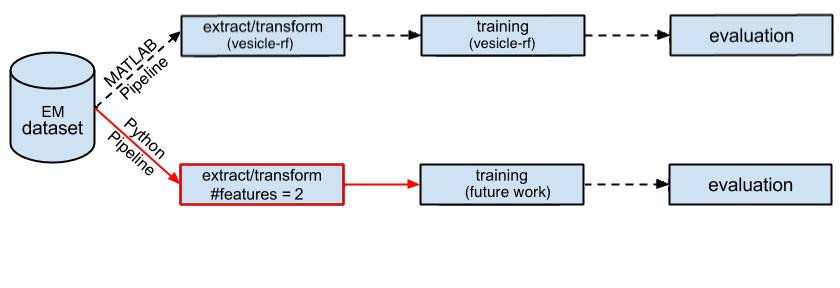
\includegraphics[scale=.5]{pipeline}
\section{Results}

Precision/Recall analysis of the existing Matlab tool was performed by first running the tool to generate annotations of a sample of EM data obtained from neurodata.io. This annotation data was then automatically compared to ground truth data assembled by hand by experts. The number of true positives, false positives, and false negatives were tallied, and led to the calculation of the following statistics:
\begin{itemize}
\item Precision: .84
\item Recall: .32
\end{itemize}
So the vesicle identification algorithm is fairly precise, but has low recall. Obviously both precision and recall have room to improve, but this performance is actually well suited to the goal of identifying synapses. On the axon side of each synapse, there is always a large number of vesicles containing neurotransmitters, so as long as a few are identified, the vesicle detection is good enough. The important thing is that there are not groups of false positive identifications clustered together, which would lead to lower precision in synapse detection; the relatively high precision makes this unlikely.

Next we began work on a similar tool in python. Two key steps are needed in the an algorithm such as ours based in computer vision. There is a feature extraction step in which potential objects you are searching for are labelled and identified. After that feature extraction “supervised learning” must be performed to train the algorithm to identify objects with precision and accuracy. In essence, multiple data sets with vesicles already identified must be fed into the algorithm and the computer will teach itself to be more accurate based on what it got right and what it got wrong.
Ultimately, we managed to build an object detection engine that extracts two features/transforms: blobdog and houghcircle.This feature extraction was the first step in the pipeline for classifying vesicles, and we yielded a very low precision of approximately .32 and a recall of approximately .77.

Our future work will involve finishing building the remainder of the pipeline depicted above by leveraging the sciki-learn library, and in particular, random forests in order to run supervised learning. This training would be done on a ground truth data compiled by experts on neuro-anatomy.


\end{document}


